\section[\textit{The Wealth of Nations} (1776)]{\textit{An Inquiry into the Nature and Causes of the Wealth of Nations} (1776)}

    Adam Smith’s seminal work laid the foundations for classical economics. Its discussion on the division of labour, the invisible hand, and self-interest has influenced economic thought for centuries.

    \subsection[Of the Principle which gives occasion to the Division of Labour]{Book I, Chapter 2 \\
                \textit{Of the Principle which gives occasion to the Division of Labour}}

        \subsubsection{The invisible hand}

            \begin{quote}
                It is not from the benevolence of the butcher, the brewer, or the baker, that we expect our dinner, but from their regard to their own interest. We address ourselves, not to their humanity but to their self-love, and never talk to them of our own necessities but of their advantages.
            \end{quote}

            This famous passage introduces the idea that individuals acting out of self-interest—rather than from any altruistic impulse—unintentionally promote the public good. Smith’s “invisible hand” suggests that as each person seeks personal advantage, society as a whole benefits from the efficient allocation of resources.

        \subsubsection{Self-interest}

            \begin{quote}
                The Wealth of Nations is a stupendous palace erected upon the granite of self-interest.

                (George Stigler, “\textit{Smith’s Travels on the Ship of State}”, 1971)
            \end{quote}

            This metaphor underscores how self-interest is not merely a personal trait but the very bedrock of economic prosperity. The image of a palace built on self-interest conveys both the strength and the inevitability of individual pursuit in shaping markets and societal wealth.

        \subsubsection{Non-tuism}

            \begin{quote}
                The economic relation does not exclude from my mind everyone but me, it potentially includes everyone but you.
                
                (Wicksteed, "\textit{The Common Sense of Political Economy}", 1910)
            \end{quote}

            Though the term “non-tuism” is uncommon, this quote highlights that while individuals focus on their own interests, the effects of their actions extend beyond themselves. Even if we consciously attend only to our own benefit, our exchanges inevitably affect others, emphasizing the interconnected nature of economic relationships.

        \subsubsection{Exchange as a tug of war}

            \begin{figure}[h]
                \centering
                \includegraphics[width=0.5\linewidth]{Images/L6-1.png}
                \label{fig:L6-1}
            \end{figure}

            The metaphor of a tug of war conveys that economic exchanges are not one-sided acts of benevolence but rather competitive, dynamic interactions. Each party pulls in a direction dictated by self-interest, and it is in the balance of these forces that mutually beneficial outcomes emerge.

    \subsection[Of the Division of Labour]{Book I, Chapter 1\\
                \textit{Of the Division of Labour}}

        \subsubsection{Advantages of the division of labour}

            \begin{quote}
                One man draws out the wire, another straights it, a third cuts it, a fourth points it, a fifth grinds it at the top for receiving the head…
            \end{quote}

            This illustration demonstrates how breaking down production into simple, repetitive tasks can vastly increase efficiency. It shows that specialization leads to:

            \begin{itemize}
                \item Increased worker dexterity
                \item Reduction of production time, eliminating the steps from one process to another
                \item Replacement of workers with machines
            \end{itemize}

            \begin{equation}
                \text{Division of Labour} \Rightarrow Exchange \xrightarrow{but \ in \ reality}{} Exchange \Rightarrow \text{Division of Labour}
            \end{equation}

            The cyclical relationship shown in the equation reflects that specialization enhances the scope for exchange, and as trade becomes more efficient, it further encourages deeper division of labour.

    \subsection[Back to "Of the Principle which gives occasion to the Division of Labour"]{Back to Book I, Chapter 2 \\
                \textit{Of the Principle which gives occasion to the Division of Labour}}

        \subsubsection{The origin of division of labour}

            \begin{quote}
                This division of labour, from which so many advantages are derived, is not originally the effect of any human wisdom, which foresees and intends that general opulence to which it gives occasion. It is the necessary, though very slow and gradual consequence of a certain propensity in human nature which has in view no such extensive utility; the propensity to truck, barter, and exchange one thing for another.
            \end{quote}

            Smith argues that specialization is not the product of deliberate planning. Instead, it is an emergent phenomenon—an unintended consequence of humans naturally engaging in trade and exchange to meet their needs.

        \subsubsection{Exchange in primitive society}

            \begin{quote}
                In a tribe of hunters or shepherds a particular person makes bows and arrows, for example, with more readiness and dexterity than any other. He frequently exchanges them for cattle or for venison with his companions; and he finds at last that he can in this manner get more cattle and venison, than if he himself went to the field to catch them. From a regard to his own interest, therefore, the making of bows and arrows grows to be his chief business, and he becomes a sort of armourer.

                Another excels in making the frames and covers of their little huts or moveable houses. He is accustomed to be of use in this way to his neighbours, who reward him in the same manner with cattle and with venison, till at last he finds it his interest to dedicate himself entirely to this employment, and to become a sort of house-carpenter.
            \end{quote}

            This passage offers an early example of specialization. As individuals discover and refine their innate talents, they gradually assume specialized roles. In doing so, they are rewarded by their community, setting the stage for more complex economic structures.

    \subsection[That the Division of Labour is limited by the Extent of the Market]{Book I, Chapter 3 \\
                \textit{That the Division of Labour is limited by the Extent of the Market}}

        \subsubsection{No nailers in a small village}

            \begin{quote}
                It is impossible there should be such a trade as even that of a nailer in the remote and inland parts of the Highlands of Scotland. Such a workman at the rate of a thousand nails a day, and three hundred working days in the year, will make three hundred thousand nails in the year. But in such a situation it would be impossible to dispose of one thousand, that is, of one day's work in the year.
            \end{quote}

            This example illustrates that the extent of market demand restricts the scope for specialization. In a small community, the volume of trade is too limited to support highly specialized professions, emphasizing that economic growth requires a sufficiently large market.

            \begin{figure}[h]
                \centering
                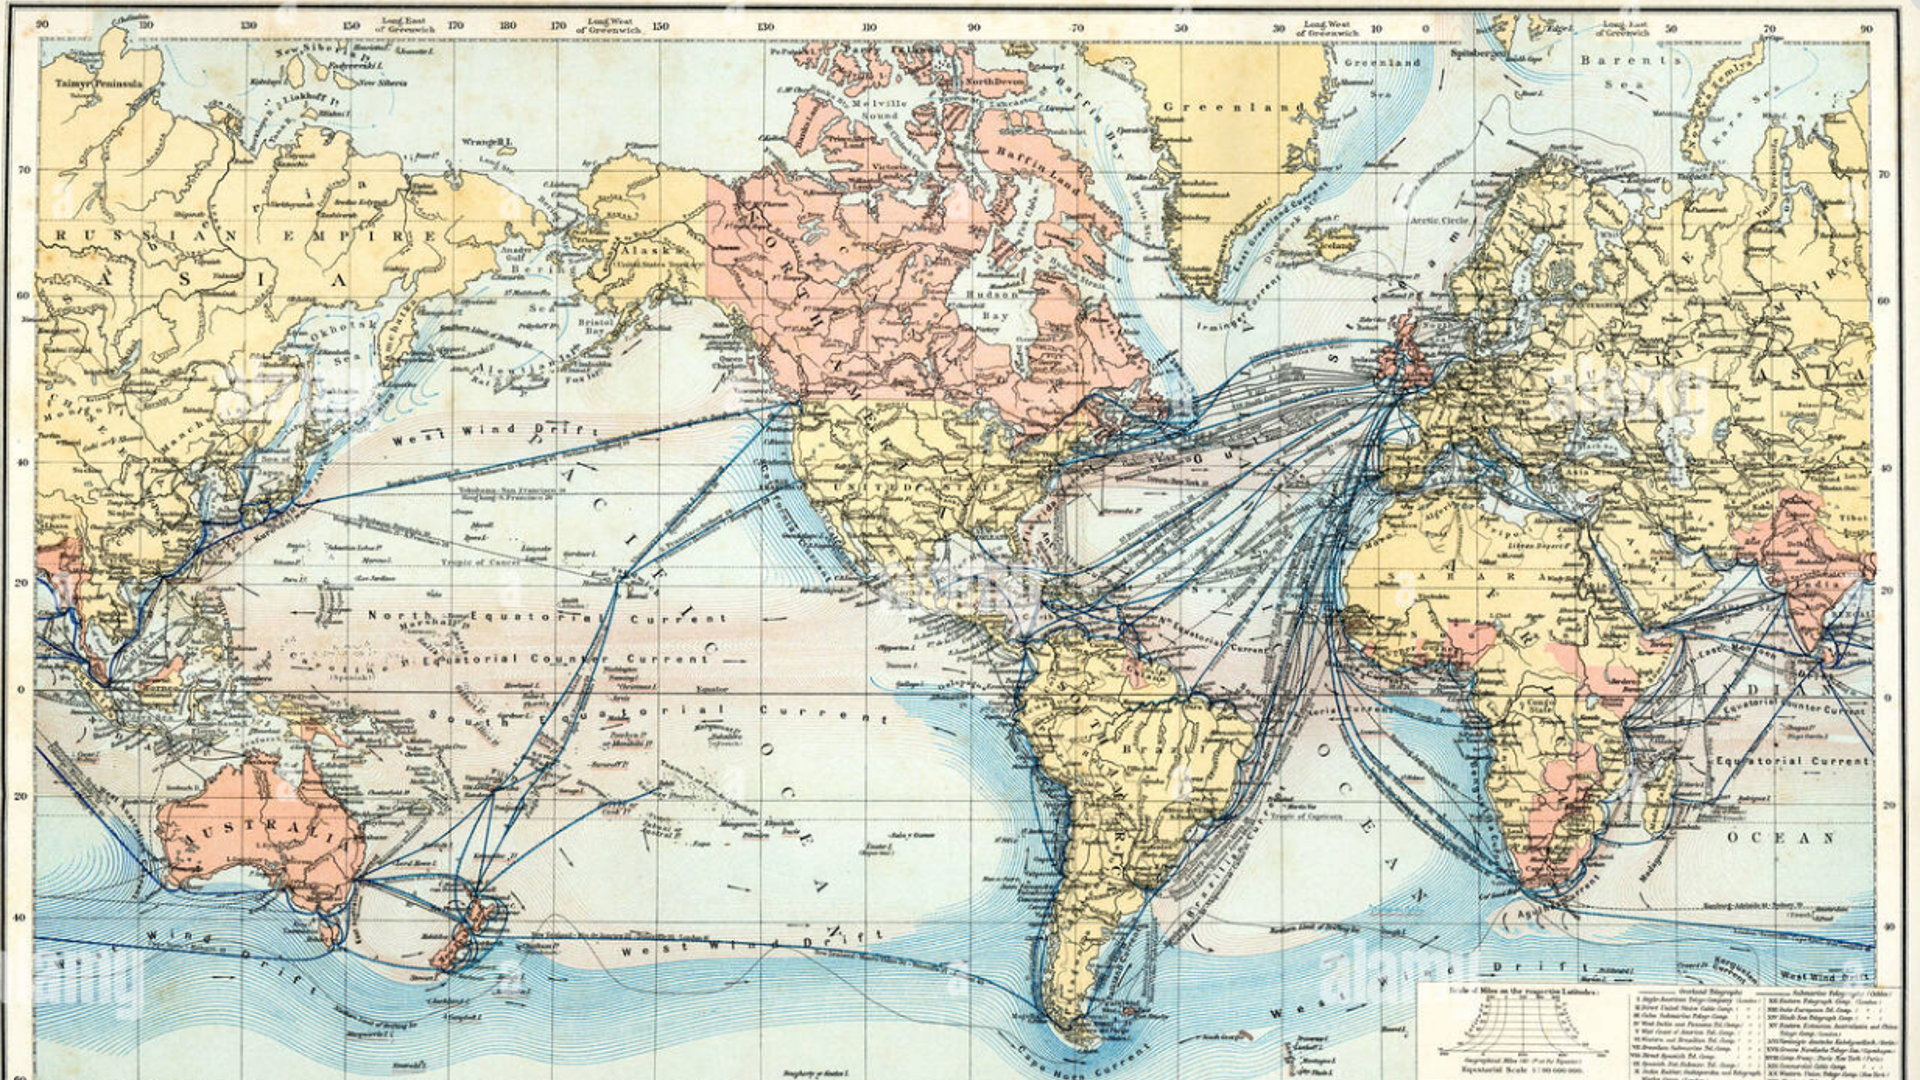
\includegraphics[width=0.75\linewidth]{Images/L6-2.png}
                \label{fig:L6-2}
            \end{figure}

    \subsection[Back to "Of the Principle which gives occasion to the Division of Labour"]{Back to Book I, Chapter 2 \\
                \textit{Of the Principle which gives occasion to the Division of Labour}}

        \subsubsection{Pursuit of one’s own interest that incidentally benefits that of others}

            \begin{quote}
                Two greyhounds, in running down the same hare, have sometimes the appearance of acting in some sort of concert. Each turns her towards his companion, or endeavours to intercept her when his companion turns her towards himself. This, however, is not the effect of any contract, but of the accidental concurrence of their passions in the same object at that particular time.
            \end{quote}

            Using the metaphor of greyhounds, Smith shows that even when individuals act independently and solely out of self-interest, their actions can coincide in a manner that appears coordinated—resulting in mutual benefit without any deliberate collaboration.

        \subsubsection{While we, the human beings}

            \begin{quote}
                We address ourselves, not to their humanity but to their \textit{self-love}, and never talk to them of our own necessities but of their advantages.
            \end{quote}

            This repetition reinforces that economic transactions are driven by self-interest. Instead of appealing to the goodwill of others, individuals structure their exchanges around what benefits both parties, even if indirectly.

        \subsubsection{Self-interest?}

            \begin{quote}
                The Wealth of Nations is a stupendous palace erected upon the granite of \textit{self-interest}.

                (George Stigler, “\textit{Smith’s Travels on the Ship of State}”, 1971)
            \end{quote}

            Within this context, the correct term is not "self-interest", but it rather is "self-love"

        \subsubsection{Egoism?}

            \begin{quote}
                Ce n’est pas de la bienveillance du boucher, du marchand de bière et du boulanger, que nous attendons notre dîner, mais bien du soin qu’ils apportent à leurs intérêts. Nous ne nous adressons pas à leur humanité, mais à leur \textit{égoïsme} ; et ce n’est jamais de nos besoins que nous leur parlons, c’est toujours de leur avantage.

                (Translated by Germain Garnier, 1802)
            \end{quote}

            \begin{remark}
                Once again, French people are making confusion: here translating "self-love" with "egoism" is incorrect, as it reduces the original meaning.
            \end{remark}

        \subsubsection{Fawning dogs}

            \begin{quote}
                When an animal wants to obtain something either of a man or of another animal, it has no other means of persuasion but to gain the favour of those whose service it requires. A puppy fawns upon its dam, and a spaniel endeavours by a thousand attractions to engage the attention of its master who is at dinner, when it wants to be fed by him.
            \end{quote}

        \subsubsection{We can’t all be friends}

            \begin{quote}
                Man sometimes uses the same arts with his brethren, and when he has no other means of engaging them to act according to his inclinations, endeavours by every servile and fawning attention to obtain their good will. He has not time, however, to do this upon every occasion. In civilized society he stands at all times in need of the cooperation and assistance of great multitudes, while his whole life is scarce sufficient to gain the friendship of a few persons.
            \end{quote}

            In large societies, deep personal bonds with everyone are impossible. Instead, individuals rely on a vast network of strangers, where market relationships replace close personal ties. This dynamic underlines the necessity of self-reliance and efficient exchange.

        \subsubsection{Human beings exchange}

            \begin{quote}
                It is not from the benevolence of the butcher, the brewer, or the baker, that we expect our dinner, but from their regard to their own interest. We address ourselves, not to their humanity but to their self-love, and never talk to them of our own necessities but of their advantages.
            \end{quote}

        \subsubsection{The beggar}

            \begin{quote}
                Nobody but a beggar chuses to depend chiefly upon the benevolence of his fellow-citizens.
            \end{quote}

\section{\textit{The Theory of Moral Sentiments} (1759)}

    \subsection{The tightrope walker}

        The analogy of the tightrope walker is used to illustrate the delicate balance between individual self-interest and the need for social approval—a balance maintained through moral sentiments.

        \subsubsection{Sympathy}

            \begin{itemize}
                \item Immediate identification
                \item Without being a “passion contagion” (David Hume)
                \item Concordance, pleasure, approval
                \item Discordance, displeasure, disapproval
                \item Theory of moral judgment based on sentiments
            \end{itemize}

            \begin{remark}
                Sympathy, for Smith, is the ability to perceive and resonate with the feelings of others. This capacity is fundamental to social cohesion, as it allows us to form moral judgments and to regulate our behavior in ways that foster mutual understanding.
            \end{remark}

        \subsubsection{The impartial spectator}

            \begin{quote}
                When I endeavour to examine my own conduct, when I endeavour to pass sentence upon it, and either to approve or condemn it, it is evident that, in all such cases, I divide myself, as it were, into two persons; and that I, the examiner and judge, represent a different character from that other I, the person whose conduct is examined into and judged of. The first is the spectator, whose sentiments with regard to my own conduct I endeavour to enter into, by placing myself in his situation, and by considering how it would appear to me, when seen from that particular point of view. The second is the agent, the person whom I properly call myself, and of whose conduct, under the character of a spectator, I was endeavouring to form some opinion. The first is the judge; the second the person judged of.
            \end{quote}

            The concept of the impartial spectator is central to Smith’s moral philosophy. It represents an internalized voice of objectivity—an imagined observer whose perspective helps us judge our own actions fairly. This mechanism encourages self-reflection and helps maintain social norms.

            \begin{minipage}{0.48\textwidth}
                \begin{center}
                    \includegraphics[width=1\linewidth]{L6-3a.png}
                    \captionof{figure}{Self-love as the pleasure of other’s approval}
                \end{center}
            \end{minipage}
            \begin{minipage}{0.04\textwidth}
                
            \end{minipage}
            \begin{minipage}{0.48\textwidth}
                \begin{center}
                    \includegraphics[width=1\linewidth]{L6-3b.png}
                    \captionof{figure}{Self-love as the pleasure of self-approval}
                \end{center}
            \end{minipage}

            \begin{figure}[h]
                \centering
                \includegraphics[width=0.32\linewidth]{L6-4.jpeg}
                \caption{Self-love as the pleasure of  deserved approval}
                \label{fig:enter-label}
            \end{figure}

        \subsubsection{The faculty of speech}

            \begin{quote}
                Whether this propensity be one of those original principles in human nature, of which no further account can be given; or whether, as seems more probable, it be the necessary consequence of the faculties of reason and speech, it belongs not to our present subject to enquire. It is common to all men, and to be found in no other race of animals, which seem to know neither this nor any other species of contracts.
                
                Nobody ever saw a dog make a fair and deliberate exchange of one bone for another with another dog. Nobody ever saw one animal by its gestures and natural cries signify to another, this is mine, that yours; I am willing to give this for that. When an animal wants to obtain something…
            \end{quote}

             This passage suggests that the faculties of reason and speech are uniquely human and have led to the development of complex social contracts and moral norms. The ability to communicate and reason underlies our capacity to negotiate, not just in economic terms, but in moral and ethical ones as well.

            \begin{proposition}
                \textbf{The pleasure of exchange:} Adam Smith’s third kind of self-love
            \end{proposition}

            This proposition encapsulates the idea that engaging in fair exchange is itself a source of satisfaction—a form of self-love that reinforces the social and economic bonds between individuals.

\section*{Additional Context and Observations}

    \begin{remark}
        Both \textit{The Wealth of Nations} and \textit{The Theory of Moral Sentiments} are best understood in the context of the Enlightenment. Smith’s work not only laid the groundwork for modern economics but also provided deep insights into human behavior, ethics, and the emergence of social institutions.
    \end{remark}

    \begin{remark}
        The juxtaposition of economic self-interest and moral sentiment is central to Smith’s philosophy. While self-interest drives market activity, the capacity for sympathy and the internal judgment of the impartial spectator help maintain social order and ethical behavior.
    \end{remark}

    \begin{remark}
        The recurring theme of self-interest—whether expressed as the invisible hand in market transactions or as the pursuit of self-approval in moral judgment—suggests that human behavior, though seemingly divided between economic and moral spheres, is underpinned by a consistent set of motivations
    \end{remark}

    \begin{remark}
        Smith’s observations about the division of labour and market size illustrate that economic specialization is both enabled and limited by the structure of society. Similarly, the development of moral sentiments is linked to the unique human capacity for language and reflection.
    \end{remark}